\documentclass{beamer}
\usepackage{beamerthemeshadow}
\usepackage{color}
\usepackage[all]{xy}


%%%% choose your presentation style:
\mode<presentation>
{
  \usetheme{Copenhagen} %%%
 \usecolortheme{beaver}

%%% set style for ovelays: lists (and other text) appearing one item at a time
%%% This will create a dimmed preview of next item:
\setbeamercovered{transparent}
%%% This will hide it entirely:
%\setbeamercovered{invisible}
}
%% if you don't want page numbers to show: 
\setbeamertemplate{footline}[page number]{}


\begin{document}
\title{Memristor Presentation}
\author{Bailey Denzer}
\institute[UMM] % (optional, but mostly needed)
{
 % \inst{1}%
  University of Minnesota, Morris
}
\date[]  
{November 12 2015}

\begin{frame}
  \titlepage
\end{frame}

\begin{frame}

  \frametitle{Outline}
\tableofcontents
\end{frame}

\section{Introduction}

\section{Background}

\subsection{Memristor}

\begin{frame}
  \frametitle{The Memristor}
  
\begin{itemize}
\item Two-terminal, non-volatile device 
\item Made of resistant $TiO_{2}$ and conductive $TiO_{2-x}$
\item Applying voltage alters the state
\end{itemize}
  
\begin{figure}
%%% note: the file is in the same folder as your .tex file
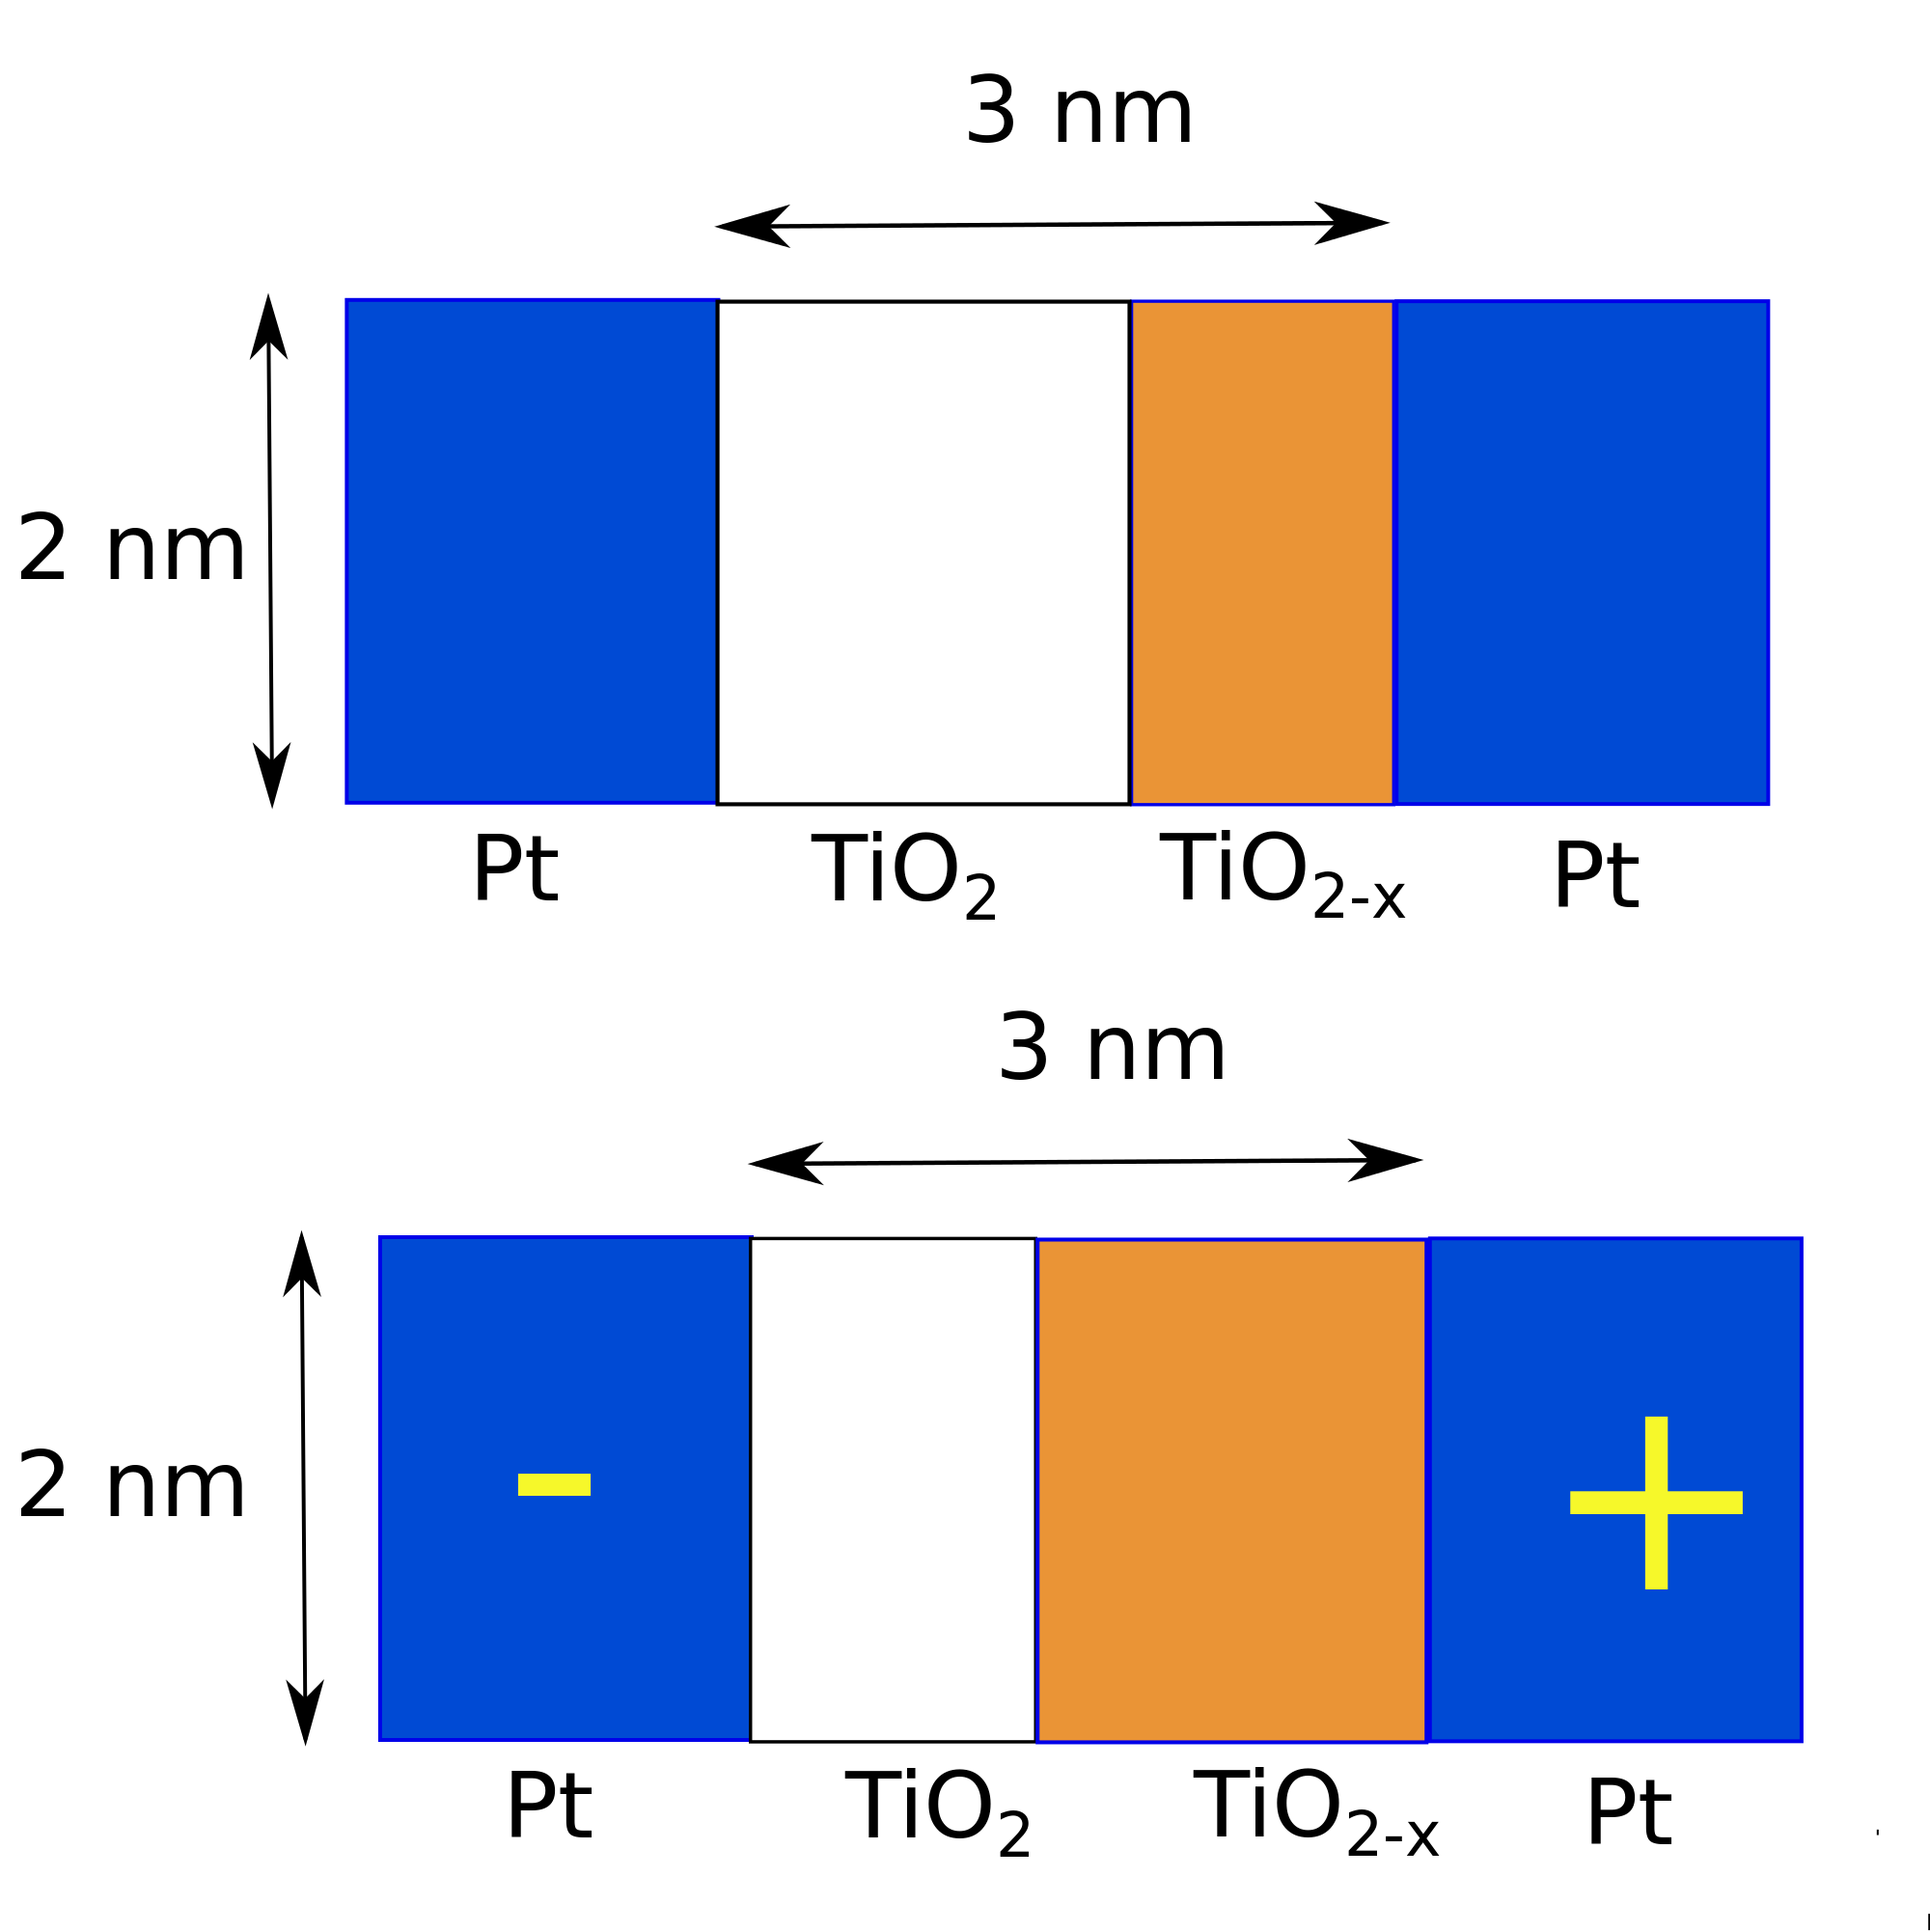
\includegraphics[height=45mmh]{memristor.png}
\end{figure}
\end{frame}

\begin{frame}
  \frametitle{Comparison to Other Memories}
  
  Not shown in the chart:
\begin{itemize}
\item Memristors are potentially cheaper to manufacture than flash.
\item DRAM energy shown does not account for refreshing.

\end{itemize}
  
\begin{figure}
%%% note: the file is in the same folder as your .tex file
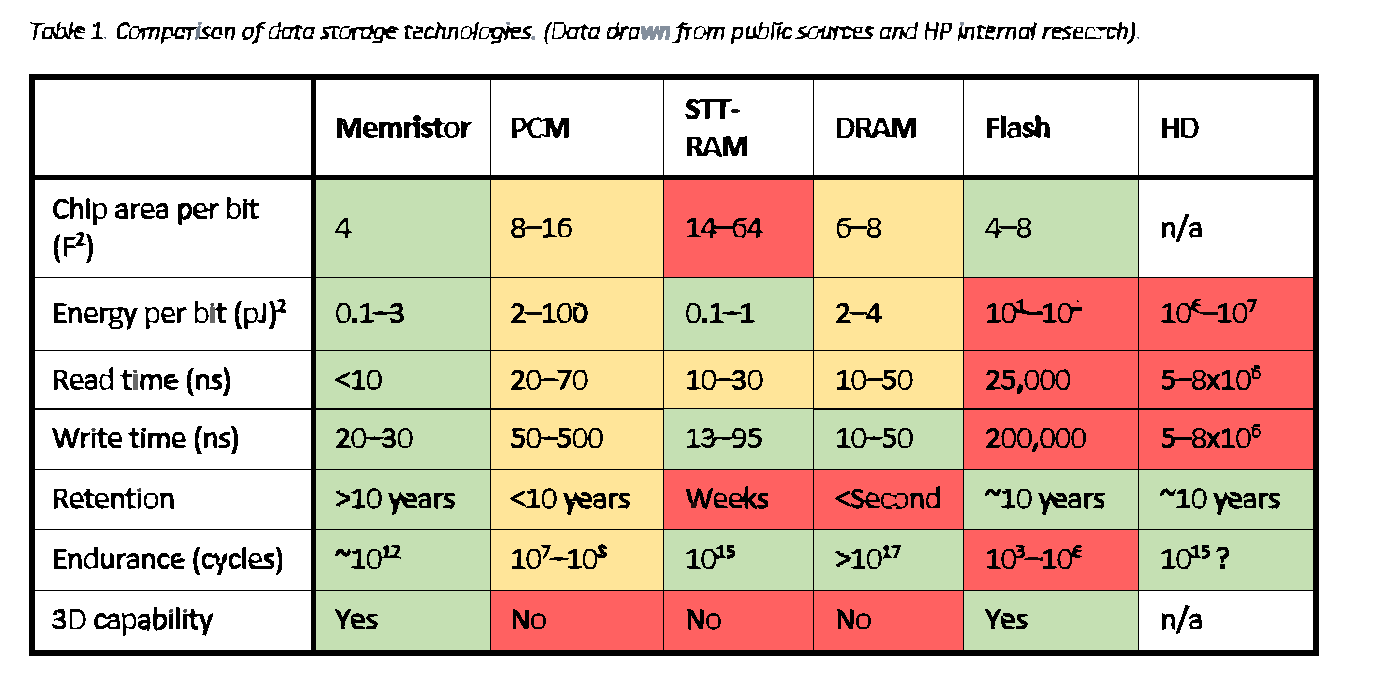
\includegraphics[height=45mmh]{Comparison-of-Data-Storage-2.pdf}
\end{figure}
\end{frame}
\subsection{Crossbar Array}

\section{Computation in Memory}

\subsection{Basic Design and IMP Logic}

\subsection{Results on Large Data Sets}

\section{Read/Write Models for a Memristor Based 1T1R Cell}

\section{Conclusion}

\begin{frame}
  \frametitle{Discussion}
Questions?
\end{frame}

\end{document}